\subsection{Общие сведения об интерференции}
Явления интерференции и дифракции -- яркое проявление волновой теории света. В этих явлениях интересны относительные значения таких фотометрических величин как: лучистый поток, световой поток, освещенность. 
Таким образом нас не будет особо интересовать конкретная фотометрическая величина, а потому введём и будем следить за \textit{интенсивностью колебаний}:
\begin{equation*}
	I = \langle\vc{E} \vc{E}^*\rangle.
\end{equation*}
Соответственно, в точке, где перекрывается два колебания электрического поля: $\vc{E} = \vc{E}_1 + \vc{E}_2$, будем иметь:
\begin{equation*}
	I = I_1 + I_2 + I_{12},
\end{equation*}
где последний член называется \textit{интерференционным членом}.
Если он обращается в нуль, то такие источники называют \textit{не когерентными}, и \textit{когерентными} иначе.

Для двух параллельных волн, введя амплитуды: $A_1 = a_1 e^{i \varphi_1}$ и для второй аналогично будем иметь:
\begin{equation*}
	E_1 = A_1 e^{i \omega t},
	\hspace{0.3 cm}
	E_2 = A_2 e^{i \omega t}
	\hspace{0.5 cm}
	\Rightarrow
	\hspace{0.5 cm}
	E = E_1 + E_2 = (A_1 + A_2)e^{i \omega t}.
\end{equation*}
Не сложно получить выражения для результирующей амплитуды и фазы:
\begin{equation*}
	a^2 = a_1^2 + a_2^2 + 2 a_1 a_2 \cos(\varphi_2 - \varphi_1),
	\hspace{1 cm}
	\tg \varphi = \frac{a_1 \sin \varphi_1 + a_2 \sin \varphi_2}{a_1 \cos \varphi_1 + a_2 \cos \varphi_2}.
\end{equation*}
То есть введя интенсивности можем убедиться в предположениях сделанных выше. Например, если фазы $\varphi_1$ и $\varphi_2$ отличаются на целое четное число $\pi$, то результирующая $I$ максимальна. Если же на нечетное число $\pi$, то $I$ минимальна:
\begin{equation*}
	I_\text{макс} = \left(\sqrt{I_1} + \sqrt{I_2}\right)^2,
	\hspace{0.5 cm}
	I_\text{макс} = \left(\sqrt{I_1} - \sqrt{I_2}\right)^2
\end{equation*}
И если $\varphi_1 - \varphi_2 = m \pi \pm \pi/2$, то $I = I_1 + I_2$. То есть наши предложения сами по себе ниче так и на самом деле вполне верны и не для параллельных лучей.


\textbf{Две плоские волны}:
\begin{equation*}
	E_1 = a_1 \cos (\omega t - \vc{k}_1  \vc{r} + \delta_1),
	\hspace{0.5 cm}
	E_2 = a_2 \cos (\omega t - \vc{k}_2  \vc{r} + \delta_2).
\end{equation*}


\begin{minipage}{0.35\textwidth}
    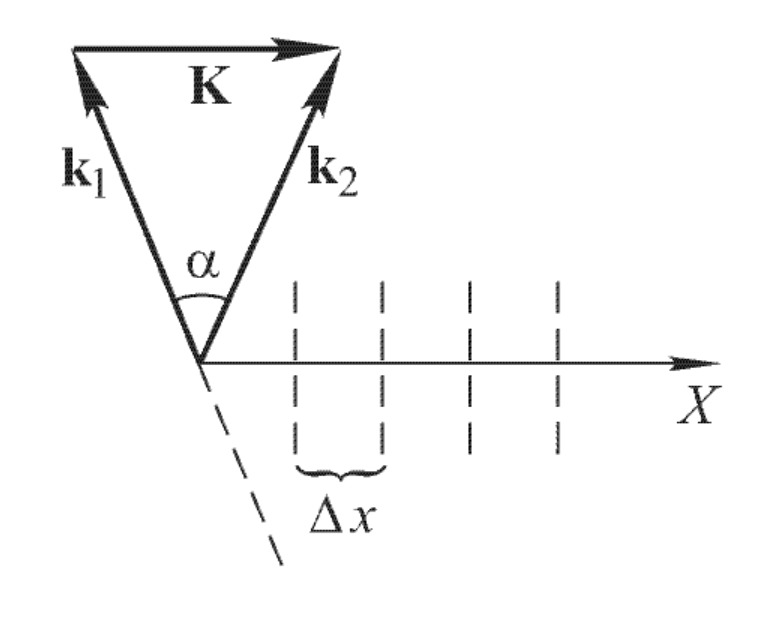
\includegraphics[width=1\textwidth]{figures/s26_1.png}
\end{minipage}
\hfill
\begin{minipage}{0.55\textwidth}
	Тут как и раньше получаем разность фаз:
	\begin{equation*}
		\varphi_2 - \varphi_1 = \vc{K} \vc{r} + (\delta_2 - \delta_1).
	\end{equation*}    
	Поверхности разных $\varphi_2 - \varphi_1 = \const$ -- плоскости обозначенные штрихами на рисунке -- параллельные $\vc{k}$. Вдоль них и результирующая интенсивность колебаний будет постоянна.
	Аналогично: максимум при четном $\pi$ для $\varphi_2 - \varphi_1$, минимум при нечетном.

	Расстояния же между соседними минимумами или максимума находится их условия
\begin{equation*}
	K \Delta x = 2 \pi.
\end{equation*}
И если $k_1 = k_2 = k = 2\pi/\lambda$. 
\end{minipage}

То находим
\begin{equation*}
	\Delta x = \frac{2 \pi}{K} = \frac{\pi}{k \sin(\alpha/2)} = \frac{\lambda}{2 \sin(\alpha/2)}
	\hspace{0.5 cm}
	\Rightarrow
	\hspace{0.5 cm}
	\Delta x \approx \frac{\lambda}{\alpha} \text{ при малых }\alpha.
\end{equation*}
Если теперь поставить плоский экран параллельно плоскости $\vc{k}_1, \vc{k}_2$, то расстояния между серединами соседних светлых(темных) полос -- \textit{ширина интерференционной полосы} будет равна $\Delta x$. Аналогично, если экран установлен перпендикулярно.
Если же теперь от перпендикулярного положения поворачивать экран, на угол $\varphi$, то ширина интерференционной полосы будет
\begin{equation*}
	\Delta_\varphi x = \Delta x / \cos \varphi.	
\end{equation*}

\text{Сферические монохроматические волны}. Будем рассматривать перекрытия волн от двух точечных источников. Амплитуда для сферической волны будет затухать обратно пропорционально $r$, то есть вдоль каждой интерференционной полосы  интенсивность будет меняться. Но мы не будем обращать внимания на это изменение.
В случае одинаковых фаз для двух источников получаем:
\begin{equation*}
	\Delta \varphi = k (r_2 - r_1) = \left(\frac{2 \pi}{\lambda}\right) (r_2 - r_1).
\end{equation*}
У нас опять светла, когда $2 m \pi$, и темна при $2 \pi (m +1/2)$. Это условие можно записать и в случае наличия сред, то есть думать надо о разности оптических путей:
\begin{equation*}
	\Delta r = r_2 - r_1 = \int n_2 d l - \int n_1 d l
	=
	\left\{
	\begin{aligned}
		m \lambda &\text{ светлая полоса}, \\
		(m+ 1/2)\lambda &\text{ темная полоса}.
	\end{aligned}
	\right.
\end{equation*}
\begin{minipage}{0.35\textwidth}
    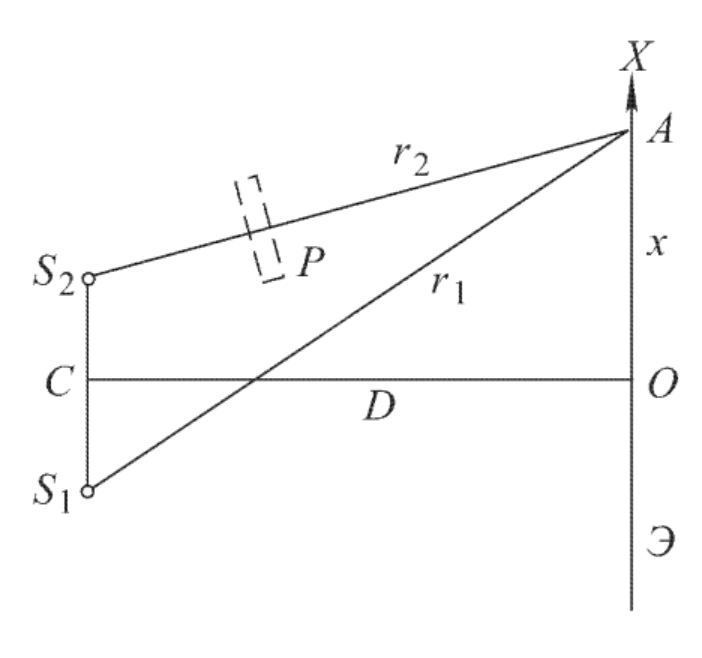
\includegraphics[width=1\textwidth]{figures/s26_2.png}
\end{minipage}
\hfill
\begin{minipage}{0.55\textwidth}
    Для наглядности приведем результаты для интерференции в такой задаче.
    \begin{equation*}
    	r_1 - r_2 = \frac{x d}{D} = \alpha x,
    \end{equation*}
    для малого угла схождения интерферирующих лучей $\alpha \approx d/D$. Для одинаковых и синфазных источников:
    \begin{equation*}
    	I = 2 I_1\left(1 + \cos \frac{2 \pi \alpha x}{\lambda}\right).
    \end{equation*}
    Ширина  интерференционной полосы $\Delta x = \lambda / \alpha$.

    Если же на пути одного из лучей поставить пластинку $P$ толщиной $l$ и с преломлением $n$, то произойдёт смещение интерференционной картины на $N = (n-1)l /\Delta x$ полос в ту сторону, с какой была введена пластинка
\end{minipage}
